
\documentstyle[color,changebar,cprog,epsbox,tabular,shadow,ascmac,graphicx]{jfspec}
\makeindex
\topmargin    -1.5cm
\headheight      1pc
\headsep         2pc
\textheight     60pc
\footskip        3pc
\footheight      1pc
\oddsidemargin   0pc
\evensidemargin  0pc
\textwidth      38pc
\columnsep       2pc
\cprogbaselineskip 1ex
\partopsep       0pc
\parsep          0pc
\itemsep         0pc
\parskip         0pc
\topsep          0pc
\renewcommand{\topfraction}{1}
\renewcommand{\floatpagefraction}{1}
\renewcommand{\dbltopfraction}{1}
\renewcommand{\dblfloatpagefraction}{1}
\renewcommand{\textfraction}{0}
\renewcommand{\bottomfraction}{0}
%\renewcommand{\floatsep}{1pc}        %$B%U%m!<%H4V$N5wN%(B
%\renewcommand{\textfloatsep}{1pc}    %$B%U%m!<%H$HK\J84V$N5wN%(B [t,b]
%\renewcommand{\dblfloatsep}{1pc}     %2$BCJAH$N>l9g$N(B \floatsep
%\renewcommand{\dbltextfloatsep}{1pc} %2$BCJAH$N>l9g$N(B \textfloatsep
%\renewcommand{\intextsep}{1pc}       %$B%U%m!<%H$HA08e$NK\J8$H$N5wN%(B [h]
\renewcommand{\indexspace}{}

\title{\shabox{\LARGE EMAX7/ACAP (IMAX3) Architecture Handbook\newline -- In-Memory Accelerator eXtension --}}
\author{Nara Institute of Science and Technology\\Computing Architecture Laboratory\\Accelerator Group}
\date{\renewcommand{\arraystretch}{0.4}\tabcolsep 0.1pc
\sboxsep=5pt \sdim=2pt \sboxrule=.4pt
\begin{tabular}{lrrr}
\multicolumn{4}{r}{EMAX7SPC-0001}\\
Ver.0.1: & Sep. &  1 & 2023\\
Ver.0.2: & Apr. &  1 & 2024\\
\end{tabular}}

\begin{document}
\maketitle
\tableofcontents
\listoffigures
\listoftables


\chapter{IMAX3 Hardware}

\section{Chiplet and Vector Length}

\begin{figure}[htbp]
\center
\includegraphics[angle=270,origin=b,width=0.85\textwidth]{fig01.eps}
\caption{\label{fig:vl}Variation of Vector Length}
\end{figure}

\begin{figure}[htbp]
\center
\includegraphics[angle=270,origin=b,width=0.32\textwidth]{fig02.eps}
\includegraphics[angle=270,origin=b,width=0.32\textwidth]{fig03.eps}
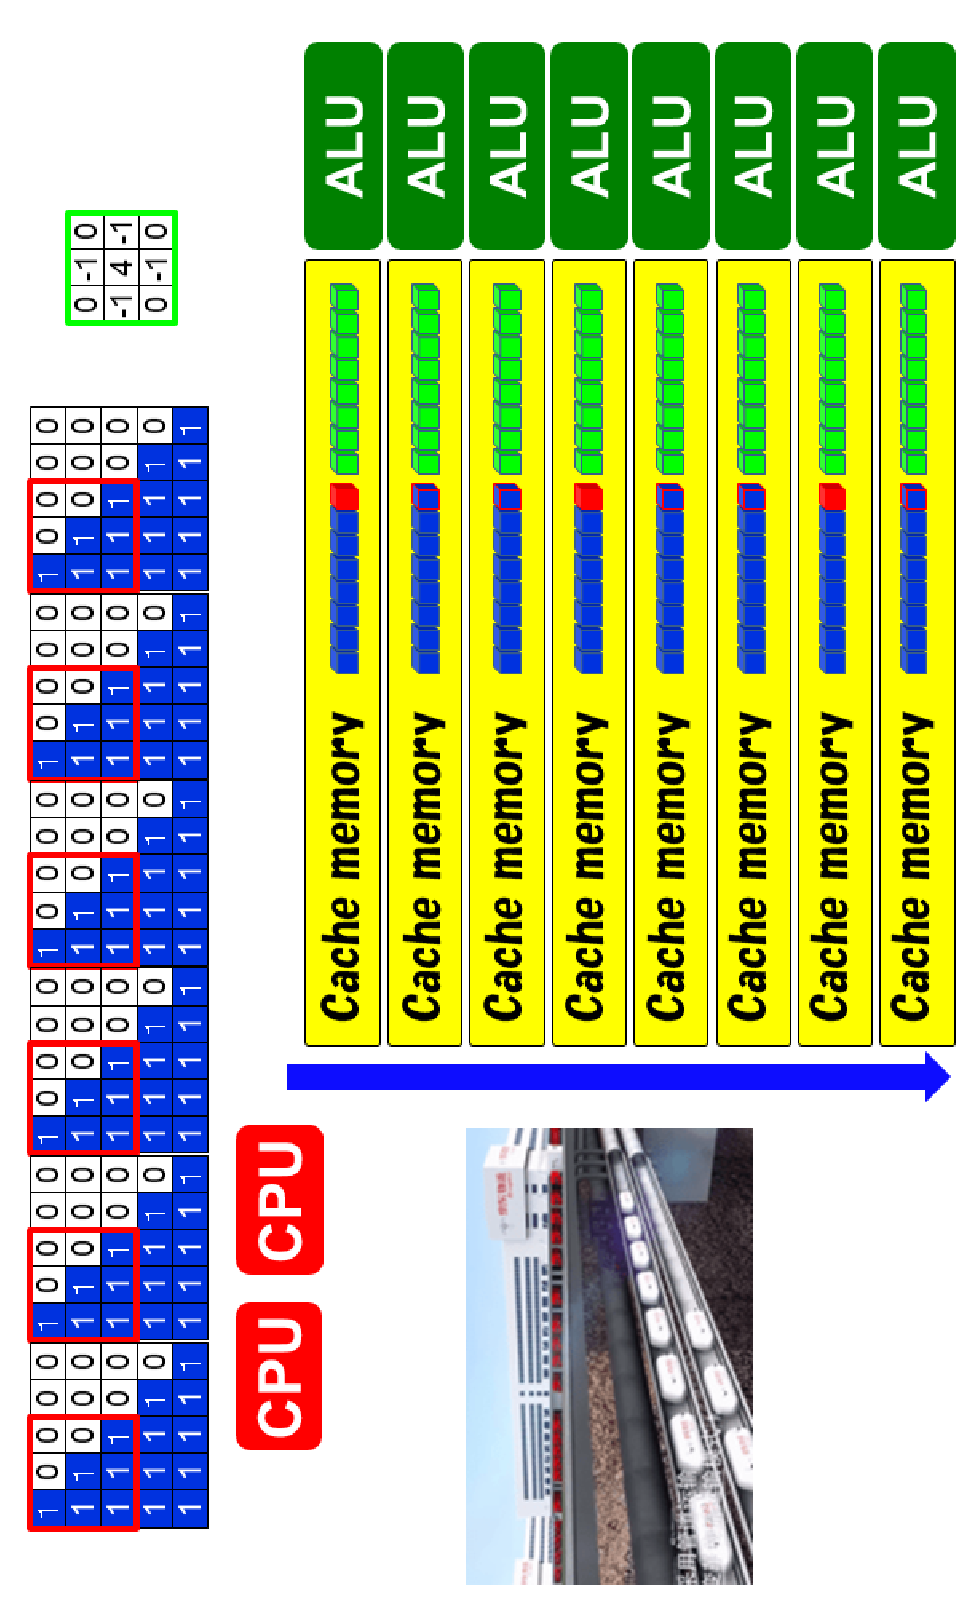
\includegraphics[angle=270,origin=b,width=0.32\textwidth]{fig04.eps}
\caption{\label{fig:comp}Multicore system, GPGPU and CGRA}
\end{figure}

Chiplets require sufficient vector length to minimize chip-to-chip data
transfer overhead. And IMAX3 is a chiplet-oriented architecture. Let's look
at the vector length in Fig.\ref{fig:vl}. A scalar processor has SIMD for
about 32 elements.  SIMD for 256 elements or more is called a vector. Vector
1 is connected to the cache memory.  Vector 2 is directly connected to the
main memory, and the vector length is about 2048.  The CGRA can have a
sandwich structure of ALU and 64KB of cache memories. The vector length is
now 16K.  By encapsulating irregular access patterns in cache memory, the
main memory can keep high speed with regular access patterns.

Figure\ref{fig:comp} illustrates typical execution models. Let's assume one
car is one CPU.  Blue data is the input image, and green data is the weight.
Every CPU tries to get the missing data in cache memory, even if it's the
same, and we cannot estimate when the data will arrive. GPGPU also has many
cores, but the cars are aligned and coalesced as much as possible before
they depart.  By merging the departure and arrival, we can reduce traffic
congestion.  However, if the destinations are scattered, GPGPU can do
nothing.  Whether coalescing is possible or not depends on the programming
skill. The right side is IMAX.  There are a few CPUs on top.  A lot of cache
memories do not go to get data and wait for the data provided by the CPU.
The CPU can send the green weight data at once.  We can reduce the amount of
data transmission and energy.

\section{Independent network for memory and execution}

\begin{figure}[htbp]
\center
\includegraphics[angle=270,origin=b,width=0.80\textwidth]{fig05.eps}
\caption{\label{fig:mesh}Execution network and Memory network}
\end{figure}

\begin{figure}[htbp]
\center
\includegraphics[angle=270,origin=b,width=0.80\textwidth]{fig06.eps}
\caption{\label{fig:ring}IMAX2 multichip structure}
\end{figure}

\begin{figure}[htbp]
\center
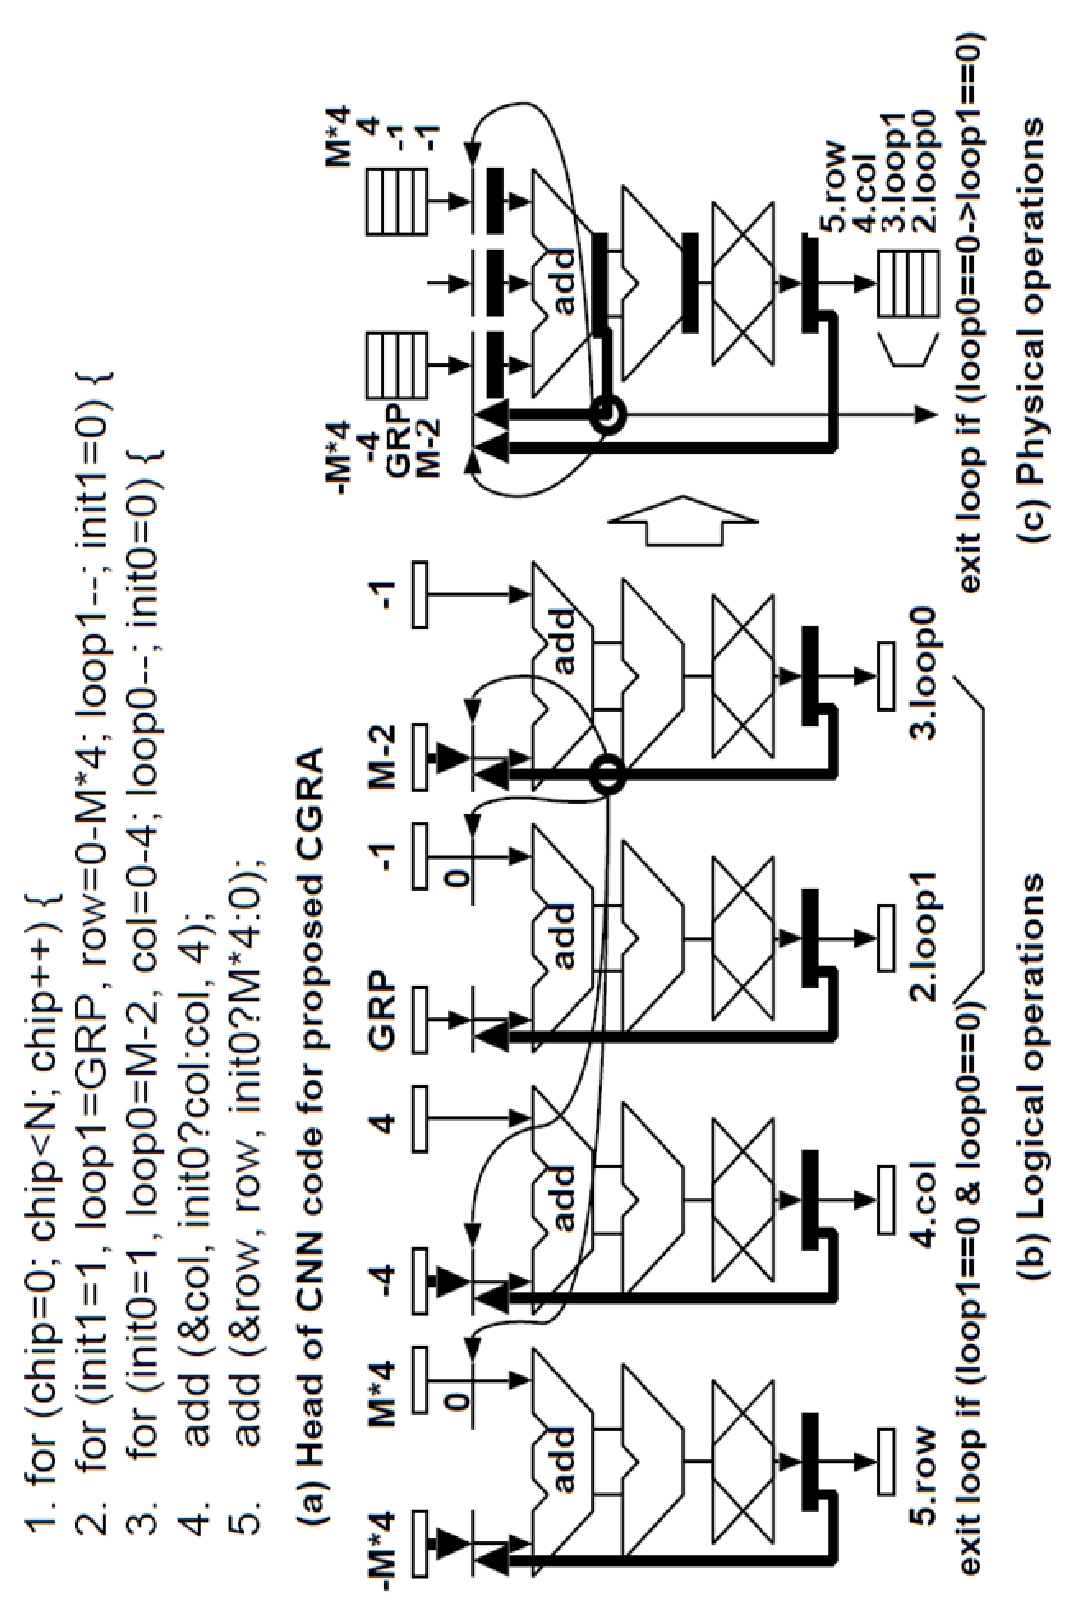
\includegraphics[angle=270,origin=b,width=0.80\textwidth]{fig30.eps}
\caption{\label{fig:loopctrl}Burst execution of triple loops}
\end{figure}

\begin{figure}[htbp]
\center
\includegraphics[angle=270,origin=b,width=0.80\textwidth]{fig33.eps}
\caption{\label{fig:multilane}IMAX3 multilane structure}
\end{figure}

As shown in Fig.\ref{fig:mesh}, there are two types of networks in
IMAX2. The latency is reduced by grouping eight units and connecting them in
parallel to the memory interface. For computation, 64 units are connected in
a ring within each chip, and the combination of computation and local memory
can be changed like a combination lock.  A ring structure is helpful for
stencil computations. By sliding the mapped operations, the pair of ALU and
cache memory can be adjusted. Much of the data in cache memory can be
reused.  To reduce the overhead, the triple loop can be mapped on IMAX as
shown in Fig.\ref{fig:ring}. The outermost loop is mapped on multiple chips,
and the inner double loop is mapped on each chip. Fig.\ref{fig:loopctrl}
illustrates how four logical units (one physical unit) manage the triple
loops. IMAX3 has multiple memory ports and multiple IMAX2 lanes, as shown
in Fig.\ref{fig:multilane}.

\section{Multilevel pipelining}

\begin{figure}[htbp]
\center
\includegraphics[angle=270,origin=b,width=0.80\textwidth]{fig07.eps}
\caption{\label{fig:micro}Micro pipelining}
\end{figure}

\begin{figure}[htbp]
\center
\includegraphics[angle=270,origin=b,width=0.80\textwidth]{fig08.eps}
\caption{\label{fig:medium}Medium pipelining}
\end{figure}

\begin{figure}[htbp]
\center
\includegraphics[angle=270,origin=b,width=0.80\textwidth]{fig09.eps}
\caption{\label{fig:macro}Macro pipelining}
\end{figure}

\begin{figure}[htbp]
\center
\includegraphics[angle=270,origin=b,width=0.80\textwidth]{fig10.eps}
\caption{\label{fig:all}Multilevel pipelining}
\end{figure}

\begin{figure}[htbp]
\center
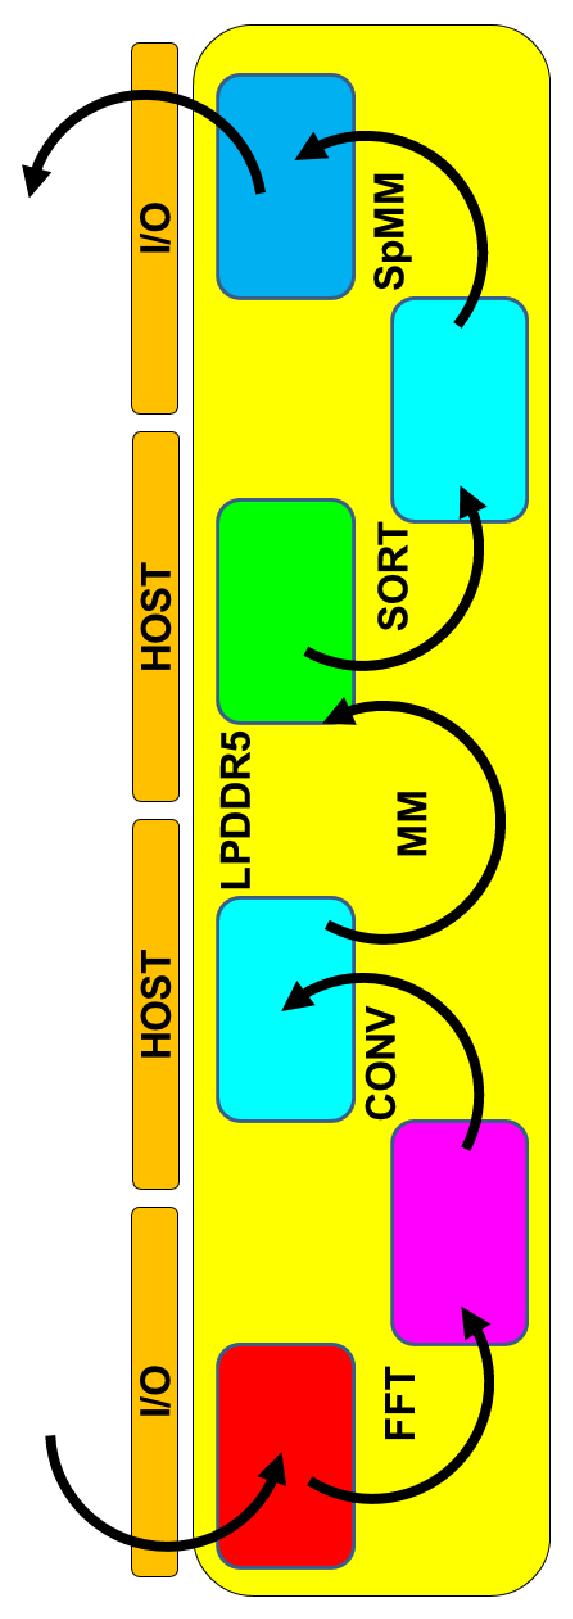
\includegraphics[angle=270,origin=b,width=0.80\textwidth]{fig11.eps}
\caption{\label{fig:map}Mapping of application kernels}
\end{figure}

Figure\ref{fig:micro} illustrates the multiple lanes of IMAX2 connected to
LPDDR5 memory, and the first level (micro) pipelining in each lane.  The micro
pipelining is the basic mode of CGRAs.  Each lane may have multiple IMAX2
chips.  This mode can follow the traditional and sequential program, and can
reduce the compilation time.  Figure\ref{fig:medium} illustrates the
multiple lanes of IMAX2 and the second level (medium) pipelining in each
lane.  The medium pipelining is provided by the double buffering in cache
memory blocks in each lane, and can follow the multiple stages in sorting,
hash function, and FFT. Figure\ref{fig:macro} illustrates the macro
pipelining of IMAX3.  The multiple lanes are concatenated as a pipeline
through LPDDR5.  Each lane may have micro and medium pipelining.
Figure\ref{fig:all} shows the final goal of IMAX3. Each lane has multiple
IMAX2 chips.  Many lanes and CPUs are employed, and many kinds of kernels
are mapped simultaneously as shown in Fig.\ref{fig:map}.

\begin{figure}[htbp]
\center
\includegraphics[angle=270,origin=b,width=0.80\textwidth]{fig12.eps}
\caption{\label{fig:chip}Area estimation}
\end{figure}

\clearpage

\section{Prototype}

\begin{figure}[htbp]
\center
\includegraphics[angle=270,origin=b,width=0.80\textwidth]{fig13.eps}
\caption{\label{fig:proto}Prototype of IMAX3}
\end{figure}

\begin{figure}[htbp]
\center
\includegraphics[angle=270,origin=b,width=0.80\textwidth]{fig14.eps}
\caption{\label{fig:evmodel}Evaluation models}
\end{figure}

As shown in Fig.\ref{fig:chip}, 75\% area of IMAX3 is memory blocks. If each
port of the LPDDR5 has four modules of 64-unit IMAX, 10240 operations can be
mapped. If 30 ports are available, 307200 operations can be mapped. If we
can fabricate with 8nm technology, 120 modules of IMAX will occupy the 144mm
square.  Figure\ref{fig:proto} is the ongoing project to scale up the IMAX2
to IMAX3. VPK180 has two sets of IMAX2 and can connect eight IMAX2 through
the NoC. Figure \ref{fig:evmodel} is a performance evaluation model using a
prototype. Eight units will be implemented: IMAX2\#0.0, IMAX2\#1.0, ...,
IMAX2\#7.0. Each IMAX2 corresponds to a configuration of NLANE=8 and NCHIP=1
in the IMAX2 application program. On the other hand, it is also possible to
run the IMAX2 application program by writing NLANE=8 and NCHIP=6. This
method corresponds to a configuration with multiple IMAX2 lanes in a cascade
configuration. However, since only the first IMAX2\#*.0 is implemented, the
execution result of subsequent IMAXs connected in cascade will be 0, and the
overhead associated with cascade connection will not be measured. The
execution speed is just a ideal value.


\chapter{IMAX3 Software}

\section{IMAX3 interface mapped on CPU memory space}

IMAX3 is just a group of multiple lanes of IMAX2 connected to a
large-capacity external memory. The hardware/software interface of IMAX3 is
a set of control interfaces for each IMAX2.

\section{Dataflow example}

\begin{figure}[htbp]
\center
\includegraphics[angle=270,origin=b,width=0.80\textwidth]{fig35.eps}
\caption{\label{fig:4dconv}Tycal series of 4D-array convolution}
\end{figure}

\begin{figure}[htbp]
\center
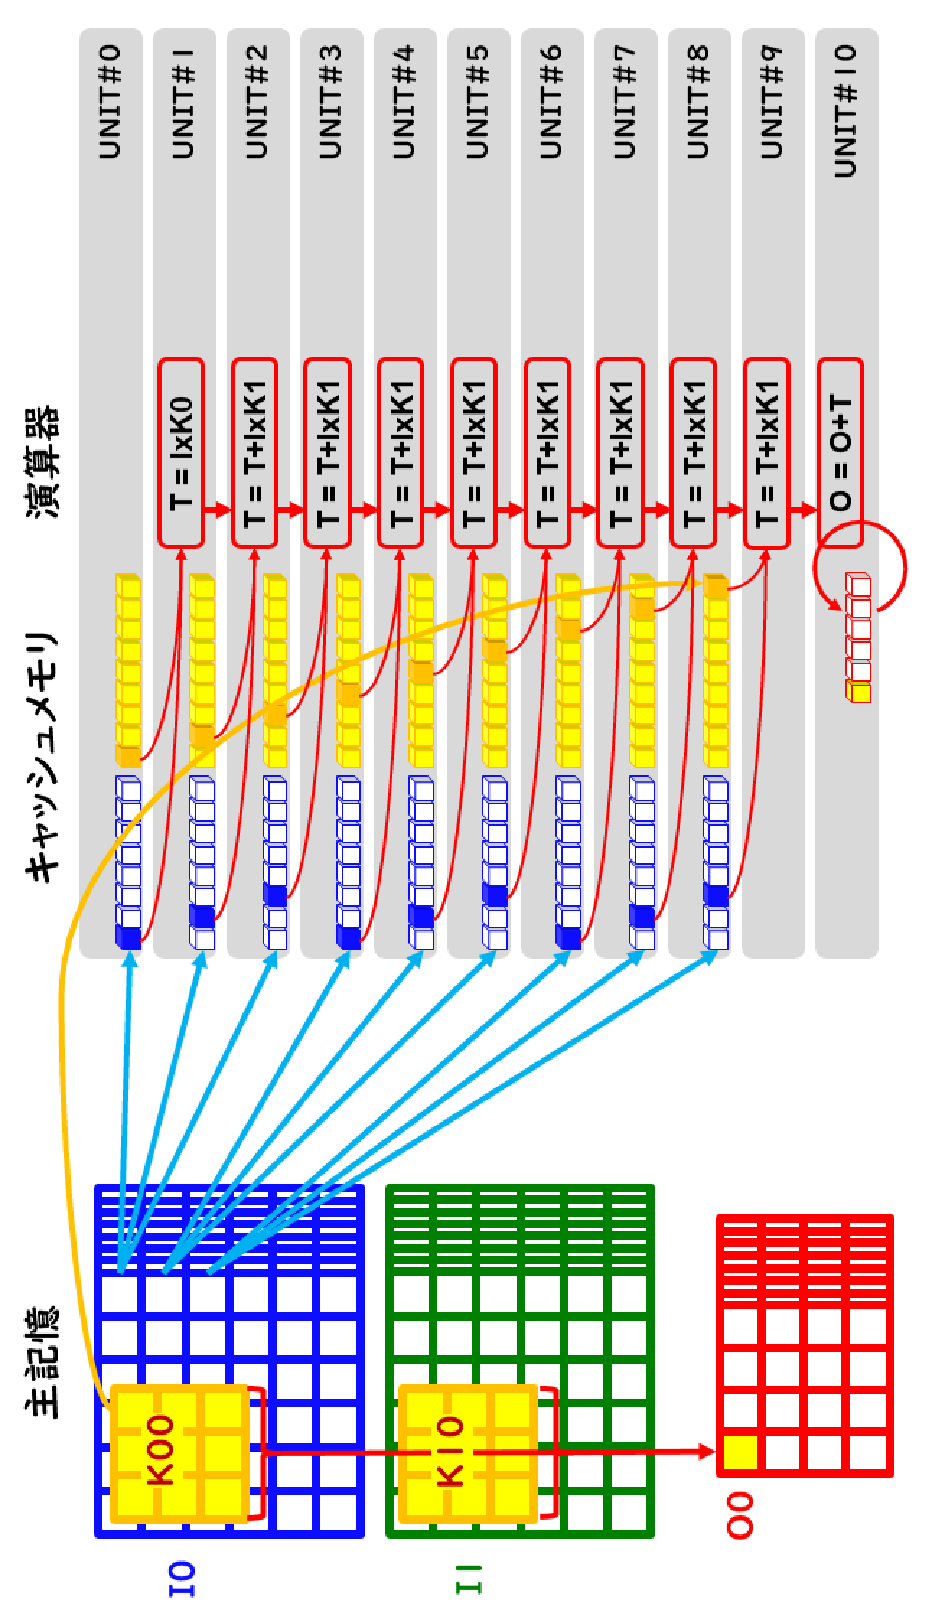
\includegraphics[angle=270,origin=b,width=0.80\textwidth]{fig36.eps}
\caption{\label{fig:4dmap}Typical mappting of convolution}
\end{figure}

\begin{figure}[htbp]
\center
\includegraphics[angle=270,origin=b,width=0.80\textwidth]{fig37.eps}
\caption{\label{fig:options}Several options to speedup convolution}
\end{figure}

\begin{figure}[htbp]
\center
\includegraphics[angle=270,origin=b,width=0.80\textwidth]{fig31.eps}
\caption{\label{fig:twoaxis}Selecting two axis from 4D array}
\end{figure}

\begin{figure}[htbp]
\center
\includegraphics[angle=270,origin=b,width=0.80\textwidth]{fig32.eps}
\caption{\label{fig:optimal}Two options to increase the length of the burst execution}
\end{figure}
 
Figure \ref{fig:4dconv} shows a typical convolution
operation. Multiplication of a part of the input data (I) and the
corresponding kernel (K), and accumulation produce the result. The shape
that 6x6 two-dimensional I0 overlap in the depth direction corresponds to
multiple 6x6 images being included in one batch. I1 has a similar structure.
For example, I0 corresponds to the blue component and I1 corresponds to the
green component. There are many pairs of input data and kernels, and the
vertical summation is the output O0. Since the input data is two-dimensional
and the calculation is repeated by shifting the kernel K in the X and Y
directions, the output O0 is also two-dimensional. Also, if you keep the
input data (I) as is and replace only the kernel (K) and perform the same
calculation, you will find another output O1. In other words, the input data
(I), kernel (K), and output data (O) are all 4-dimensional
arrays. Furthermore, in the multilayer convolution operation, the same
calculation is repeated using the output data (O) as the next input data
(I).

There are several ways to perform the above convolution operations using
IMAX3. Fig.\ref{fig:4dmap} is the basic form of two-dimensional convolution.
Each IMAX unit contains cache memory and a computing unit that are
controlled by the host driver. Blue input data in main memory is broadcast
to the blue part of the cache memory, and yellow kernels in main memory are
broadcast to the yellow part. Unit 0 extracts the data corresponding to the
upper left corner of the kernel and sends it to unit 1. Unit 1 performs the
multiplication and sends the result to unit 2. By connecting the above,
finally, unit 10 accumulates the sum of the 9 multiplication results to the
red output, and completes one 3x3 convolution operation. All units perform
calculations one after another while shifting the input data to the right,
and the output data is updated continuously. The above is a typical CGRA
calculation method.

A feature of IMAX is the large number of degrees of freedom in combining the
above basic shapes according to the size of the 4-dimensional array
(Fig.\ref{fig:options}). The goal of optimization is to reduce execution
time, and the methods are broadcasting and maximum reuse of cache
memory. One chip of IMAX2 can continuously execute double loops at once, and
can map four sets of convolution operations into a logical four-column
structure. What remains is which axis of the 4-dimensional data should be
mapped to the double loop. Once you decide which axis of input I to select,
the others will be determined automatically, so first select the axis of
blue input data (I). There are four candidates: the X axis, Y axis, batch
axis, and channel axis, as shown in Fig.\ref{fig:twoaxis}. However, the
X-axis should be selected because the addresses are continuous. Similarly,
the channel axis is efficient if used to fill 64 units, so the remaining
axes have two choices: the Y axis or the batch axis.

Figure\ref{fig:optimal} shows two mapping methods. When using the X and Y
axes, the yellow data does not need to be reshaped because it is a
continuous address. It is most efficient if the data size of one sheet,
which is the product of the length of X and the length of Y, is stored in
the cache memory within the unit. For example, if the cache memory is
16Kwords, it can accommodate up to 128x128. In the case of 256x256, you can
keep this format and divide it into four in the Y direction. On the other
hand, after multilayer convolution, the result is a small square such as
2x2, which shortens IMAX's continuous execution time and increases startup
overhead. In such cases, use the batch axis instead of the Y axis. Although
the overhead associated with reshaping increases, if the number of batches
is 100, it becomes 2x100, which allows the data size to be increased and the
startup overhead to be reduced. In the case of 3D convolution, you can
similarly increase the continuous operation time of IMAX and reduce the
number of startups.

\section{Programming model of Macro pipelining}

\begin{figure}[htbp]
\center
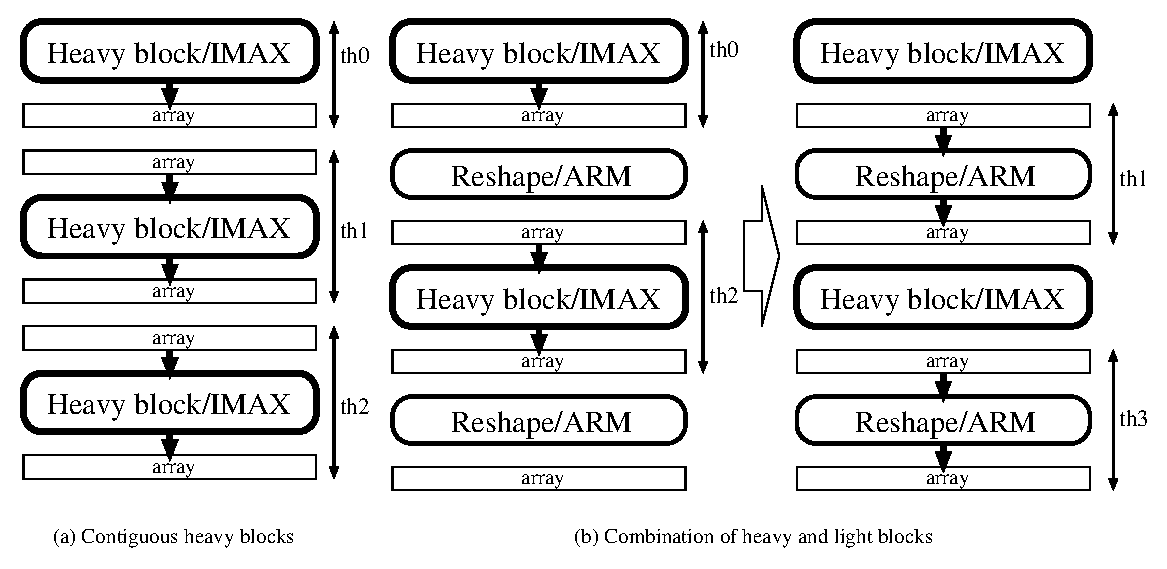
\includegraphics[angle=0,origin=b,width=0.85\textwidth]{macro-pipe.eps}
\caption{\label{fig:model0}Programming model}
\end{figure}

Figure\ref{fig:model0} is the programming model related to macro pipelining. 
In (a), there are three sections with long processing times, and the macro
pipelining is performed. The main thread starts three threads and speeds up
each section using IMAX. A double buffer is required for the data structure
between threads so that the input and output of each thread do not
interfere. On the other hand, (b) is a case where the long processing time
is executed by IMAX, but there is short-term processing by the host, such as
exchanging array indexes, between the heavy processing. By using short-time
processing as a double buffer, memory usage can be reduced compared to
applying double buffers between all threads.

\section{Programming style of Macro pipelining}

\begin{figure}[htbp]
\center
\includegraphics[angle=270,origin=b,width=0.85\textwidth]{fig15.eps}
\caption{\label{fig:model1}Programming style}
\end{figure}

Figure\ref{fig:model1} is the programming style. For the macro pipelining,
multiple threads are started, and the function (th\_inference) containing
the loop structure is executed in parallel. The th\_inference() repeatedly
executes nn\_forward(), which simulates a multilayer CNN. Although
nn\_forward() is executed simultaneously by multiple threads, each thread
executes only the part it is responsible for, and performs pipeline
processing while waiting to complete processing in the previous and
subsequent layers. In each layer, function calls that take LANE as an
argument use IMAX2. Multiple HOSTs and IMAX2 participate in macro
pipelining.  By using sigwait() instead of a busy loops, waiting between
threads can be performed on HOST even if HOST does not have enough cores.


\chapter{Examples}

\section{Image Recognition (tsim)}

MNIST

\shabox{
\leftline{cent\% make -f Makefile-cent.emax7nc all clean}
\leftline{cent\% cd ../; tsim/tsim-cent.emax7nc -x -t -I0 -C1 -F1}
}

\shabox{
\leftline{acap\% make -f Makefile-acap.emax7+dma all clean}
\leftline{acap\% cd ../; tsim/tsim-acap.emax7+dma -x -t -I0 -C1 -F1}
}

\vskip .1in

CIFAR10

\shabox{
\leftline{cent\% make -f Makefile-cent.emax7nc all clean}
\leftline{cent\% cd ../; tsim/tsim-cent.emax7nc -x -t -I1 -C6 -F2}
}

\shabox{
\leftline{acap\% make -f Makefile-acap.emax7+dma all clean}
\leftline{acap\% cd ../; tsim/tsim-acap.emax7+dma -x -t -I1 -C6 -F2}
}

\begin{figure}[htbp]
\center
\includegraphics[angle=270,origin=b,width=0.80\textwidth]{ssim.eps}
\caption{Image recognition (training + inference)}
\end{figure}

\clearpage

\subsection{Header}

IMAX3 uses ARM's multithreading to control multiple IMAX2 lanes. NTHREAD is
the number of threads to be activated in ARM when multiple IMAX2 lanes are
activated. EMAX\_LANE is the upper limit of the control variable set to
control the IMAX2 lanes activated simultaneously. Also, NLANE is the number
of IMAX2 lanes detected in the actual machine. IMAX2 detected in the real
machine over EMAX\_LANE is not used. In other words, the value set in NLANE
is always less than or equal to EMAX\_LANE. Note that NTHREAD must be
greater than or equal to NLANE.

\begin{screen}
\scriptsize
\begin{verbatim}
#define MAX_NTHREAD 16
volatile struct th_inference_args {
  int      thid;
  int      stat;     /* 0:idle, 1:run, 2:wait (enq/deq, DMA, EXEC) */
  sigset_t sigset;   /* sys/_sigset.h 2B/4B */
  int      deq;
  int      enq;
  float4D *slice;
  CNNet   *net;
  int      batch_size;
  int      nchan;
  int      insize;
} th_inference_args[MAX_NTHREAD];
volatile int th_inference_retv[MAX_NTHREAD];
pthread_t    th_inference_t[MAX_NTHREAD];
void         th_inference(struct th_inference_args *);
\end{verbatim}
\end{screen}

\subsection{IMAX3 thread driver}

When launching multiple IMAX2 and configuring a macro pipeline, prepare a
function wrapper (th\_inference in the example below) that includes the IMAX2
kernel, and use ARM's pthread\_create to launch NTHREAD threads. Thread
arguments include thread number and enq/deq for pipeline synchronization.

\begin{screen}
\scriptsize
\begin{verbatim}
  int THREAD;
  for (THREAD=0; THREAD<NTHREAD; THREAD++) {
    th_inference_args[THREAD].thid       = THREAD;
    th_inference_args[THREAD].stat       = 1; /* run */
    sigemptyset(&th_inference_args[THREAD].sigset);
    sigaddset(&th_inference_args[THREAD].sigset, SIGUSR1);
    pthread_sigmask(SIG_BLOCK, &th_inference_args[THREAD].sigset, NULL);
    th_inference_args[THREAD].enq        = 0;
    th_inference_args[THREAD].deq        = 0;
    th_inference_args[THREAD].slice      = &slice;
    th_inference_args[THREAD].net        = net;
    th_inference_args[THREAD].batch_size = batch_size;
    th_inference_args[THREAD].nchan      = nchan;
    th_inference_args[THREAD].insize     = insize;
  }
  if (NTHREAD > 1) {
    for (THREAD=0; THREAD<NTHREAD; THREAD++)
      pthread_create(&th_inference_t[THREAD], NULL, (void*)th_inference, &th_inference_args[THREAD]); /* 0-(NTHREAD-1) */
    while (1) {
      int cont = 0;
      usleep(4000); /* 4msec 2024/01/24 Nakashima */
      for (THREAD=0; THREAD<NTHREAD; THREAD++) {
        switch (th_inference_args[THREAD].stat) {
        case 0:            break;/* idle */
        case 1:  cont = 1; break;/* run */
        default: cont = 1; pthread_kill(th_inference_t[THREAD], SIGUSR1); break; /* wait */
        }
      }
      if (!cont) break;
    }
    for (THREAD=0; THREAD<NTHREAD; THREAD++)
      pthread_join(th_inference_t[THREAD], NULL);
  }
  else {
    for (THREAD=0; THREAD<NTHREAD; THREAD++)
      th_inference(&th_inference_args[THREAD]);
  }
\end{verbatim}
\end{screen}

\clearpage

\subsection{IMAX3 thread wrapper}

Multiple wrappers are started at the same time. In order for multiple
threads to work in the pipeline internally, the code should be wrriten to
execute the part in charge based on the thread number given as an argument.

\begin{screen}
\scriptsize
\begin{verbatim}
/* IMAX3 MACROPIPELIING for EVALUATION */
void th_inference(struct th_inference_args *args)
{
  int THREAD     = args->thid;
  float4D *slice = args->slice;
  CNNet *net     = args->net;
  int batch_size = args->batch_size;
  int nchan      = args->nchan;
  int insize     = args->insize;
  int j, k;
  /************************************/
  /* TARGET of MACRO-PIPELINING/IMAX3 */
  /************************************/
  slice->nstrides = batch_size;
  slice->nchannel = xtest.nchannel;
  slice->kstrides = xtest.kstrides;
  slice->stride_size = xtest.stride_size;
  for (j=0; j+batch_size<=xtest.nstrides; j+=batch_size) {
    if (THREAD == 0) {
      slice->data = &(xtest.data[j*xtest.stride_size*xtest.kstrides*xtest.nchannel]);
      if (cnn_mode) {
        if (enable_x11) {
          F4i2Ipl(batch_size, nchan, insize, insize, I, slice); /* 100batch x 28x28 x 1chan */
          copy_I_to_BGR(D, batch_size, insize, insize, I);
          BGR_to_X(0, D);
        }
        // copy data to input layer
        copy4D(&(net->ninput), slice);
        if (attn_mode) {
          attention(&(net->ninput), &(net->work), &(net->attention)); /* batch,RGB,H,W */
          if (enable_x11) {
            F4i2Ipl(batch_size, nchan, insize, insize, I, &(net->work)); /* 100batch x 28x28 x 1chan */
            copy_I_to_BGR(D, batch_size, insize, insize, I);
            BGR_to_X(3, D);
            F4i2Ipl(batch_size, nchan, insize, insize, I, &(net->ninput)); /* 100batch x 28x28 x 1chan */
            copy_I_to_BGR(D, batch_size, insize, insize, I);
            BGR_to_X(1, D);
          }
        }
      }
      if (eye_mode) {
        F4i2Ipl(batch_size, nchan, insize, insize, I, slice); /* 100batch x 28x28 x 1chan */
        copy_I_to_BGR(R, batch_size, insize, insize, I); /* R <- I */
        copy_I_to_BGR(L, batch_size, insize, insize, I); /* L <- I */
        if (enable_x11)
          BGR_to_X(0, R);
        /* pre-processing by eye-model */
        eyemodel(enable_x11, slit_type); /* L+R -> Sl+Sr */
        /* import Sr to hidden_layer */
        Ipl2F4h(10, WD, HT, Sr, Cr, R, &net->nhidden[0]); /* 100batch x 24x24 x 9chan -> hidden */
      }
    }
    nn_forward(/*MACROPIPE*/1, THREAD, net, c[input_type], f[input_type], &pred, spike_mode);
    if ((NTHREAD==1 || eye_mode)
      ||(CNN_DEPTH==1 && THREAD==2)
      ||(CNN_DEPTH==3 && THREAD==6)
      ||(CNN_DEPTH==4 && THREAD==8)
      ||(CNN_DEPTH==6 && THREAD==12)) {

      for (k=0;k<batch_size;k++) {
        float *A = &(pred.data[k*pred.stride_size]);
        nerr += (MaxIndex(A, pred.stride_size) != ytest[j+k]);
      }
      if (enable_x11) {
        clear_BGR(D);
        copy_H_to_BGR(D+WD*(HT*1/4), &net->nhidden[0]);
        copy_H_to_BGR(D+WD*(HT*2/4), &net->nhidden[CNN_DEPTH-1]);
        BGR_to_X(2, D);
        while (x11_checkevent());
      }
    }
  }
  /*********************************/
  /* END of MACRO-PIPELINING/IMAX3 */
  /*********************************/
  args->stat = 0; /* idle */
}
\end{verbatim}
\end{screen}

\clearpage

\subsection{IMAX3 region}

The nn\_forward below is the top-level function that performs the
inference. Currently, the argument THREAD is manually associated with the
IMAX2 lane number (LANE) to be used. In addition, enq/deq is used to
synchronize the macro pipeline. In the future, when automation tools are
completed, manual work will be unnecessary.

\begin{screen}
\scriptsize
\begin{verbatim}
void nn_forward(int MACROPIPE, int THREAD, CNNet *net, struct c *c, struct f *f, float2D *oubatch, int spike_mode)
{ /* NTHREAD 1:MACRO_PIPE_OFF 2-:MACRO_PIPE_ON */
  /*                             EMAX7:NTHREAD=8 other:NTHREAD=1 */
  /*                              ZYNQ:NLANE=X                   */
  /*                              othr:NLANE=4                   */
  /* train:     nn_forward(0, 1)                                 */
  /* inference: nn_forward(1, T)                                 */
  /* camera:    nn_forward(0, 1)                                 */
  /* th#>0�ξ��,����enq==deq�ʤ��Ե� �ǽ�th#̤���ξ��,����enq!=deq�ʤ��Ե� */
  /* �Ե����֤ˤʤ����,����deq=1-deq�˹���                                  */
  /* ����enq�Ǽ��Ȥ�dbuf����                                                 */
  /* �Ǹ��,            ����enq=1-enq�˹���                                  */
  /* DBUF��                                                              */
  /* th#0      ****0* ****1* ****2*  CNN0:ninput->nhidden[0]                 */
  /*      enq 0     11     00     11                                         */
  /*      deq 0     01     10     01                                         */
  /* th#1     -------*0*    *1*    *2*  nhidden[0]->npool[0]                 */
  /*      enq 0        11     00     11                                      */
  /*      deq 0        01     10     01                                      */
  /* th#2     ----------****0* ****1* ****2*  CNN1:npool[0]->nhidden[1]      */
  /*      enq 0              11     00     11                                */
  /*      deq 0              01     10     01                                */
  /* th#3     ----------------*0*    *1*    *2*  nhidden[1]->npool[1]        */

  /* NHIDDEN/NPOOL��DBUF�Ȥ��ƻȤ����                                       */
  /* th#0      ****0*  ****1*  ****2*  CNN0:ninput->nhidden[0]               */
  /*      enq 0     1 1     0 0     1 1                                      */
  /*      deq 0     0 1     1 0     0 1                                      */
  /* th#1     ------*0*     *1*     *2*  nhidden[0]->npool[0]                */
  /*      enq 0       1     1 0     0 1                                      */
  /*      deq 0       0     1 1     0 0     1                                */
  /* th#2     ---------****0*  ****1*  ****2*  CNN1:npool[0]->nhidden[1]     */
  /*      enq 0             1 1     0 0     1 1                              */
  /*      deq 0             0 1     1 0     0 1                              */
  /* th#3     --------------*0*     *1*     *2*  nhidden[1]->npool[1]        */

  int batch_size = net->ninput.nstrides;
  int i, j, k, l;
  float *temp;

  if (cnn_mode && !(CNN_DEPTH==1 && FC_DEPTH==1) && !(CNN_DEPTH==3 && FC_DEPTH==1)
               && !(CNN_DEPTH==4 && FC_DEPTH==1) && !(CNN_DEPTH==6 && FC_DEPTH==2)) { /* IGNORE MACRO_PIPE in cnn_mode */
    if (THREAD > 0) exit(0);
  }
  if (eye_mode) { /* IGNORE MACRO_PIPE in eye_mode */
    if (THREAD > 0) exit(0);
  }
  if (spike_mode) { /* IGNORE MACRO_PIPE in spike_mode */
    if (THREAD > 0) exit(0);
  }
  if (spike_mode) {
    /* SMAX1 assumes -V* -C1 */
    // add bias broadcast<2>(hbias, hidden.shape);
    temp = net->nhidden[0].data;
    for (i=0;i<net->nhidden[0].nstrides;i++) {
      for (j=0;j<net->nhidden[0].nchannel;j++) {
        for (k=0;k<net->nhidden[0].kstrides*net->nhidden[0].stride_size;k++,temp++)
          *temp += net->hbias[0].data[j];
      }
    }
    relu4(&(net->nhidden[0]));                                                 /* V1->c.nhidden[0].data */
    max_pooling(&(net->npool[0]), &(net->nhidden[0]), c[0].psize, c[0].psize); /*   ->c.npool[0].data */
    flat4Dto2D(&(net->nflat[0]), &(net->npool[0]));                            /*   ->f.nflat[0].data */
    smax_trial(0, net, c, f); /* IGNORE MACRO_PIPE */
  }
\end{verbatim}
\end{screen}

\begin{screen}
\scriptsize
\begin{verbatim}
  else {
    int LANE = 0;
    for (l=0; l<CNN_DEPTH; l++) {
      /***************************************************************************/
      if (!MACROPIPE || NTHREAD==1 || eye_mode) {}
      else if (THREAD == l*2) {
        if (THREAD>0) while (th_inference_args[THREAD-1].enq==th_inference_args[THREAD-1].deq) { inference_sigwait; }
                      while (th_inference_args[THREAD  ].enq!=th_inference_args[THREAD  ].deq) { inference_sigwait; }
        //th_inference_args[THREAD-1].deq = 1-th_inference_args[THREAD-1].deq; /* DBUF�� */
#if defined(EMAX7)
        if (l >= NLANE) {
          printf("nn_forward_CNN: LANE(%d) >= NLANE(%d)\n", l, NLANE);
          exit(1);
        }
        LANE = l;
        emax7[LANE].sigwait = 1; /* ON */
        emax7[LANE].sigstat = &th_inference_args[THREAD].stat;
        emax7[LANE].sigset  = &th_inference_args[THREAD].sigset;
#endif
      }
      else
        goto end_of_cnn; /* skip other task */
      /***************************************************************************/
      if (l>0 || cnn_mode) {
        // first layer, conv, use stride=2
        /***********************ninput*** V CNN    */
#ifndef CUDA
/*��IMAX3��*/conv_forward(THREAD, LANE, l==0?&(net->ninput):&(net->npool[l-1]), &(net->Ki2h[l]),
                          &(net->nhidden[l]), c[l].ksize, &(net->tmp_col[l]), &(net->tmp_dst[l]));
#else
        conv_forward_cuda(l==0?&(net->ninput):&(net->npool[l-1]), &(net->Ki2h[l]),
                          &(net->nhidden[l]), c[l].ksize, &(net->tmp_col[l]), &(net->tmp_dst[l]));
#endif
      }

      // add bias broadcast<2>(hbias, hidden.shape);
      temp = net->nhidden[l].data;
      for (i=0;i<net->nhidden[l].nstrides;i++) {
        for (j=0;j<net->nhidden[l].nchannel;j++) {
          for (k=0;k<net->nhidden[l].kstrides*net->nhidden[l].stride_size;k++,temp++)
            *temp += net->hbias[l].data[j];
        }
      }
      // Activation, relu, backup activation in nhidden
      // nhidden = F<relu>(nhidden);
      relu4(&(net->nhidden[l]));
      copy4D(&(net->nhiddenbak[l]), &(net->nhidden[l]));

      /***************************************************************************/
      if (!MACROPIPE || NTHREAD==1 || eye_mode) {
      }
      else if (THREAD == l*2) {
        if (THREAD>0) th_inference_args[THREAD-1].deq = 1-th_inference_args[THREAD-1].deq;
                      th_inference_args[THREAD  ].enq = 1-th_inference_args[THREAD  ].enq;
      }
      /***************************************************************************/
    end_of_cnn:
\end{verbatim}
\end{screen}

\begin{screen}
\scriptsize
\begin{verbatim}
      /***************************************************************************/
      if (!MACROPIPE || NTHREAD==1 || eye_mode) {
      }
      else if (THREAD == l*2+1) {
        while (th_inference_args[THREAD-1].enq==th_inference_args[THREAD-1].deq) { inference_sigwait; }
        while (th_inference_args[THREAD  ].enq!=th_inference_args[THREAD  ].deq) { inference_sigwait; }
        //th_inference_args[THREAD-1].deq = 1-th_inference_args[THREAD-1].deq; /* DBUF�� */
      }
      else
        goto end_of_maxpool; /* skip other task */
      /***************************************************************************/

      // max pooling /*����nhidden���������鳫��*/
      max_pooling(&(net->npool[l]), &(net->nhidden[l]), c[l].psize, c[l].psize);
      copy4D(&(net->npoolbak[l]), &(net->npool[l]));

      /***************************************************************************/
      if (!MACROPIPE || NTHREAD==1 || eye_mode) {
      }
      else if (THREAD == l*2+1) {
        th_inference_args[THREAD-1].deq = 1-th_inference_args[THREAD-1].deq; /* NHIDDEN/NPOOL��Ȥä�DBUF�ξ�� */
        th_inference_args[THREAD  ].enq = 1-th_inference_args[THREAD  ].enq;
      }
      /***************************************************************************/
    end_of_maxpool:
      continue;
    }
\end{verbatim}
\end{screen}

\begin{screen}
\scriptsize
\begin{verbatim}
    /***************************************************************************/
    if (!MACROPIPE || NTHREAD==1 || eye_mode)
      LANE = 0;
    else if (THREAD == CNN_DEPTH*2) {
      while (th_inference_args[THREAD-1].enq==th_inference_args[THREAD-1].deq) { inference_sigwait; }
      //th_inference_args[THREAD-1].deq = 1-th_inference_args[THREAD-1].deq; /* DBUF�� */
#if defined(EMAX7)
      if (CNN_DEPTH >= NLANE) {
        printf("nn_forward_FC: CNN_DEPTH(%d) >= NLANE(%d)\n", CNN_DEPTH, NLANE);
        exit(1);
      }
      LANE = CNN_DEPTH;
      emax7[LANE].sigwait = 1; /* ON */
      emax7[LANE].sigstat = &th_inference_args[THREAD].stat;
      emax7[LANE].sigset  = &th_inference_args[THREAD].sigset;
#endif
    }
    else
      goto end_of_fc; /* skip other task */
    /***************************************************************************/
    for (l=0; l<FC_DEPTH; l++) {
      if (l==0)                                                  /***********************npool**** A CNN    */
        flat4Dto2D(&(net->nflat[0]), &(net->npool[CNN_DEPTH-1]));/*************************|****** BOUNDARY */
      else                                                       /***********************nflat**** V FC     */
        copy2D(&(net->nflat[l]), &(net->nout[l-1]));

      // second layer full-connection
/*��IMAX3��*/multiply_float2D(THREAD, LANE, &(net->nout[l]), &(net->nflat[l]), 0, &(net->Wh2o[l]), 0);
      repmat_add(&(net->nout[l]), &(net->obias[l]), batch_size);

      if (l < FC_DEPTH-1) {
        // activation, sigmloid, backup activation in fhidden
#if 1
        sigmoid(&(net->nout[l]));
#else
        relu2(&(net->nout[l]));
#endif
        copy2D(&(net->noutbak[l]), &(net->nout[l]));
      }
      else { /* l == FC_DEPTH-1 */
        // softmax calculation
        softmax2D(&(net->nout[FC_DEPTH-1]), &(net->nout[FC_DEPTH-1]));
      }
    }
    /***************************************************************************/
    if (!MACROPIPE || NTHREAD==1 || eye_mode)   {
    }
    else if (THREAD == CNN_DEPTH*2)
      th_inference_args[THREAD-1].deq = 1-th_inference_args[THREAD-1].deq; /* NHIDDEN/NPOOL��Ȥä�DBUF�ξ�� */
    /***************************************************************************/
    end_of_fc:;
  }

  if ((!MACROPIPE || NTHREAD==1 || eye_mode)
    ||(CNN_DEPTH==1 && THREAD==2)
    ||(CNN_DEPTH==3 && THREAD==6)
    ||(CNN_DEPTH==4 && THREAD==8)
    ||(CNN_DEPTH==6 && THREAD==12)
      ) {
    // copy result out
    copy2D( oubatch, &(net->nout[FC_DEPTH-1]));
  }
}
\end{verbatim}
\end{screen}

%%


\chapter{Appendix}

\section{References}

This chapter lists related specifications, standards, references, related source programs, and tool chains.

\begin{itemize}
\parskip 0pc \itemsep 0pc
\item EMAX5 Basic patent                                           \dotfill proj-arm64/doc/pat35.tgz
\item IMAX Basic patent                                            \dotfill proj-arm64/doc/pat36.tgz
\parskip 0pc \itemsep 0pc
\item ARMv8 Architecture specification                             \dotfill proj-arm64/doc/arm/DDI0487A\_f\_armv8\_arm.pdf
\item ARM Cortex-A53 MPCore Processor Technical Reference Manual\\ \dotfill proj-arm64/doc/arm/ARM-CORTEX-A53\_R0P4.pdf
\item ZYNQ Ultrascale+ SoC Technical Reference Manual\\            \dotfill proj-board/zcu102/doc/ug1085-zynq-ultrascale-trm.pdf
\item AMBA AXI4 and ACE Protocol Specification                     \dotfill proj-arm64/doc/arm/AXI4\_specification.pdf
\item IMAX3 Handbook                                               \dotfill proj-arm64/doc/emax7/emax7e.pdf
\item IMAX3 Preprocessor                                           \dotfill proj-arm64/src/conv-c2d/conv-c2d
\item IMAX2 Handbook                                               \dotfill proj-arm64/doc/emax6/emax6e.pdf
\item IMAX2 Preprocessor                                           \dotfill proj-arm64/src/conv-c2c/conv-c2c
\item IMAX2 SImulator                                              \dotfill proj-arm64/src/csim/csim
\item Example(3x3-2D cnn)                                          \dotfill proj-arm64/sample/mm\_cnn\_if/cnn+rmm.c
\item Example(3x3-3D cnn)                                          \dotfill proj-arm64/sample/mm\_cnn\_if/cnn3d+rmm.c
\item Example(MM)                                                  \dotfill proj-arm64/sample/mm\_cnn\_if/mm+rmm.c
\item Example(Inverse matrix��                                     \dotfill proj-arm64/sample/mm\_cnn\_if/inv+rmm.c
\item Example(Lightfield rendering)                                \dotfill proj-arm64/sample/mm\_cnn\_if/gather+rmm.c
\item Example(Lightfield depth map)                                \dotfill proj-arm64/sample/mm\_cnn\_if/gdepth+rmm.c
\item Example(Image recognition+stochastic ALU)                    \dotfill proj-arm64/sample/tsim/imax.c
\item Example(Chat GPT)                                            \dotfill proj-arm64/sample/vsim/imax.c
\end{itemize}


\end{document}
